\documentclass[12pt, a4paper, onecolumn]{article} 
\usepackage[utf8]{inputenc}
\usepackage{fancyhdr}
\usepackage{graphicx}
\usepackage{geometry}
\usepackage{float}
\usepackage{multicol} 
\usepackage{lmodern}  
\usepackage[T1]{fontenc}  
\usepackage{hyperref}  
\usepackage[dvipsnames]{xcolor}  % Enable predefined colors
\usepackage{listings, lstautogobble}
\usepackage{listings}


\definecolor{codegreen}{rgb}{0,0.6,0}
\definecolor{codegray}{rgb}{0.5,0.5,0.5}
\definecolor{codepurple}{rgb}{0.58,0,0.82}
\definecolor{backcolour}{rgb}{0.95,0.95,0.92}

\lstdefinestyle{mystyle}{
	backgroundcolor=\color{backcolour},   
	commentstyle=\color{codegreen},
	keywordstyle=\color{magenta},
	numberstyle=\tiny\color{codegray},
	stringstyle=\color{codepurple},
	basicstyle=\ttfamily\footnotesize,
	breakatwhitespace=false,         
	breaklines=true,                 
	captionpos=b,                    
	keepspaces=true,                 
	numbers=left,                    
	numbersep=5pt,                  
	showspaces=false,                
	showstringspaces=false,
	showtabs=false,                  
	tabsize=2
}

% Réduire les marges
\geometry{top=1.5cm, bottom=1.5cm, left=1.5cm, right=1.5cm}

\input{structure.tex} 

%----------------------------------------------------------------------------------------
%	ARTICLE INFORMATION
%----------------------------------------------------------------------------------------

\title{Labo7 - POO \\ Calculatrice} 

% Modifiez le style des auteurs
\newcommand{\largename}[1]{{\Large\textbf{#1}}} % style pour le nom de famille

\author{
	\authorstyle{Dani Tiago \largename{Faria dos Santos}\\ Antoine \largename{Aubry } \\ \\ Groupe  \textbf{L02GrP}\\ HEIG-VD} % Authors
}

\makeatletter
\renewcommand\date[1]{\gdef\@date{\hbox to \linewidth{#1\hss}}}
\makeatother
\date{\today}


\pagestyle{fancy}
\fancyhf{}
\fancyhead[L]{Laboratoire 7 - POO}
\fancyhead[R]{Groupe L03GrD}
\fancyfoot[R]{Page \thepage}
\fancyfoot[L]{HEIG-VD | Dani Tiago \textbf{Faria dos Santos} - Antoine \textbf{Aubry }}



% Ligne sous l'en-tête
\renewcommand{\headrulewidth}{0.7pt}
% Pas de ligne sur le pied de page
\renewcommand{\footrulewidth}{0.5pt}


\begin{document}
	% Utilisation de twocolumn pour le titre
	\twocolumn[ 
	\maketitle
	]
	
	% Retour à une seule colonne
	\onecolumn 
	
	% Table des matières
	\tableofcontents
	\newpage
	
	
	\section{Choix de conception}
\subsection{Operator}

\begin{flushleft}
	Pour la classe \texttt{Operator}, nous avons décidé de créer une hiérarchie en concevant des sous-classes abstraites pour chaque type d'opération. Cela permet de structurer et d'optimiser les opérations selon le principe de la séparation des responsabilités. Par exemple, la méthode \texttt{Digit()} est dédiée à la création d'un entier correspondant au bouton numérique pressé. Une fois le chiffre saisi, il est directement affiché via la méthode publique \texttt{update()}. Cette approche rend le code plus modulaire et facilite l'ajout de nouvelles fonctionnalités ou d'opérations dans le futur.
\linebreak

Chaque sous-classe implémente les comportements spécifiques à une opération donnée. Cela inclut les opérateurs arithmétiques de base (\texttt{Add}, \texttt{Subtract}, \texttt{Multiply}, \texttt{Divide}) ainsi que d'autres fonctionnalités comme la gestion des pourcentages, des puissances ou des opérations spécifiques définies par l'utilisateur.
\end{flushleft}

\subsection{State}

\begin{flushleft}
	La classe \texttt{State} est responsable de la gestion des valeurs et de la pile (\texttt{Stack}). Elle joue un rôle central dans la manipulation des données et leur affichage sur l'application Calculatrice. Voici ses principales responsabilités :
\end{flushleft}

\begin{itemize}
\item \textbf{Gestion de la valeur affichée :} \\
La variable publique \texttt{value}, de type \texttt{String}, représente le contenu actuellement affiché sur l'écran de la calculatrice. Les méthodes publiques de \texttt{State} permettent d'accéder directement à cette variable et de la modifier en fonction des actions effectuées par l'utilisateur.

\item \textbf{Vérifications et gestion des erreurs :} \\
Des méthodes spécifiques permettent de vérifier si un objet existe ou si sa valeur est \texttt{null}. Cela garantit une manipulation sécurisée des données et évite les erreurs inattendues lors de l'exécution.

\item \textbf{Interaction avec la pile (\texttt{Stack}) :} \\
La pile est utilisée pour gérer les opérations complexes nécessitant un stockage temporaire de valeurs intermédiaires. Des méthodes privées sont mises en place pour permettre à la classe \texttt{State} de vérifier et de manipuler l'état de la \texttt{Stack} sans exposer directement son contenu. Cette encapsulation renforce la sécurité et la robustesse de la logique.

\item \textbf{Extensions et modularité :} \\
La classe \texttt{State} est conçue de manière extensible, permettant d'ajouter de nouvelles fonctionnalités ou de modifier le comportement existant sans compromettre la stabilité du système. Par exemple, des méthodes pourraient être ajoutées pour prendre en charge des formats d'entrée plus complexes (nombres décimaux, exposants, etc.).
\end{itemize}


	
\section{Modélisation UML}
\subsection{Diagramme des classes}
\begin{figure}[H]
	\centering
	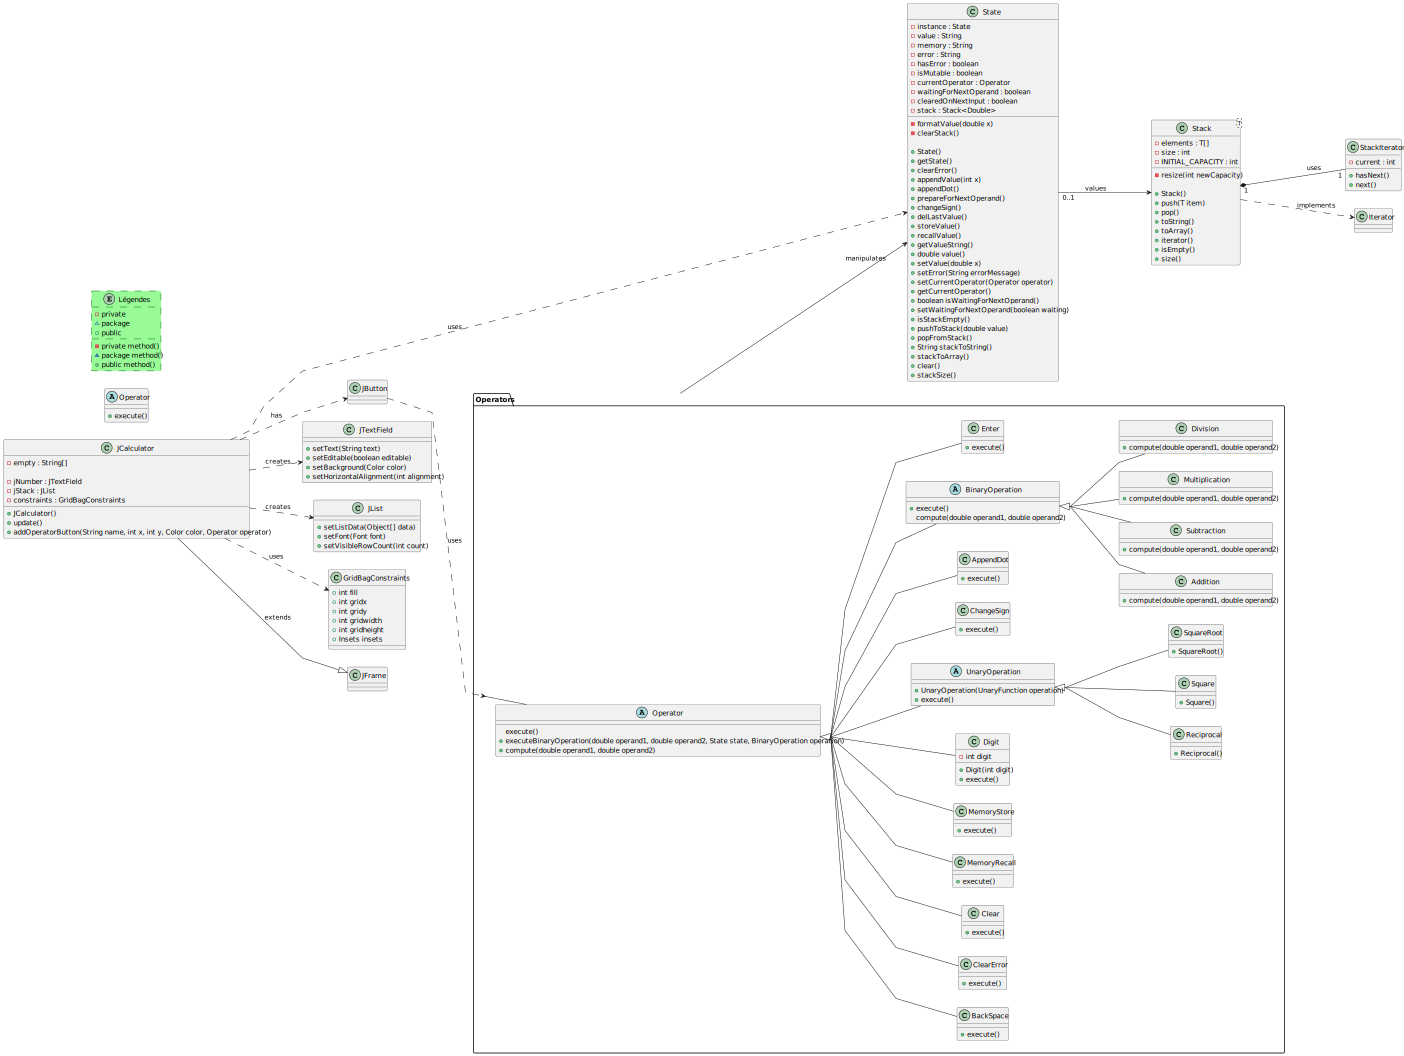
\includegraphics[width=1.1\textwidth]{../UML_Diagrams/diagram_final.jpeg}
	\caption{Implémentation de la modélisation de la Calculatrice}
\end{figure}

\pagebreak

\section{Tests}

Les tests suivants ont été réalisés pour valider les fonctionnalités principales de la calculatrice. 

\subsection{Stack}
\begin{itemize}
	\item \textbf{Étape 1 : Empiler des valeurs et tester} \\
	Valeurs empilées : 10.0 et 5.0. \\
	Résultat attendu : \texttt{[5.0, 10.0]} \\
	Résultat obtenu : \texttt{[5.0, 10.0]} \\
	\textbf{Test réussi.}
\end{itemize}

\subsection{Addition}
\begin{itemize}
	\item \textbf{Étape 2 : Addition (10 + 5)} \\
	Opération : Addition des deux valeurs empilées. \\
	Résultat attendu : \texttt{[15.0]} \\
	Résultat obtenu : \texttt{[15.0]} \\
	\textbf{Test réussi.}
\end{itemize}

\subsection{Multiplication}
\begin{itemize}
	\item \textbf{Étape 3 : Empiler une nouvelle valeur et multiplier} \\
	Valeur ajoutée : 3.0. \\
	Opération : Multiplication (15.0 * 3.0). \\
	Résultat attendu : \texttt{[45.0]} \\
	Résultat obtenu : \texttt{[45.0]} \\
	\textbf{Test réussi.}
\end{itemize}

\subsection{Division}
\begin{itemize}
	\item \textbf{Étape 4 : Diviser par une nouvelle valeur} \\
	Valeur ajoutée : 9.0. \\
	Opération : Division (45.0 / 9.0). \\
	Résultat attendu : \texttt{[5.0]} \\
	Résultat obtenu : \texttt{[5.0]} \\
	\textbf{Test réussi.}
\end{itemize}

\subsection{Opérations avancées}
\begin{itemize}
	\item \textbf{Étape 5 : Racine carrée} \\
	Valeur ajoutée : 4.0. \\
	Opération : Racine carrée de 4.0. \\
	Résultat attendu : \texttt{[2.0, 5.0]} \\
	Résultat obtenu : \texttt{[2.0, 5.0]} \\
	\textbf{Test réussi.}
	\\
	\item \textbf{Étape 6 : Mise au carré} \\
	Opération : Mise au carré du sommet de la pile (2.0). \\
	Résultat attendu : \texttt{[4.0, 5.0]} \\
	Résultat obtenu : \texttt{[4.0, 5.0]} \\
	\textbf{Test réussi.}
	\\
	\item \textbf{Étape 7 : Inverse (1/x)} \\
	Opération : Calcul de l'inverse (1/4.0). \\
	Résultat attendu : \texttt{[0.25, 5.0]} \\
	Résultat obtenu : \texttt{[0.25, 5.0]} \\
	\textbf{Test réussi.}
	\\
	\item \textbf{Étape 8 : Combinaison complexe} \\
	Valeur ajoutée : 2.0. \\
	Opérations : Multiplication (0.25 * 2.0), ajout de 5.0, soustraction. \\
	Résultat attendu : \texttt{[-4.5, 5.0]} \\
	Résultat obtenu : \texttt{[-4.5, 5.0]} \\
	\textbf{Test réussi.}
\end{itemize}

\subsection{Réinitialisation}
\begin{itemize}
	\item \textbf{Étape 9 : Réinitialisation de la pile} \\
	Opération : Effacement complet de la pile. \\
	Résultat attendu : \texttt{[]} \\
	Résultat obtenu : \texttt{[]} \\
	\textbf{Test réussi.}
\end{itemize}

\subsection{Résumé des résultats}
Tous les tests ont été exécutés avec succès, validant ainsi les principales fonctionnalités de la calculatrice, y compris les opérations arithmétiques de base, les opérations avancées, et la gestion correcte de l'état interne.


\end{document}
